% Gabarit pandoc des corrigés publiés (brut et guidé). Contenu sans marque ni nom de site.
% Compilation : lualatex (latexmk -lualatex).
% Le Markdown reste la source unique : ne pas éditer ce fichier .tex à la main.
\documentclass[11pt,a4paper]{article}

% --- Moteur, polices (Latin Modern) et langue ---------------------------------
\usepackage{iftex}
\ifLuaTeX\else\errmessage{Ce document se compile avec lualatex}\fi
\usepackage{amsmath,amssymb,mathtools}
\usepackage{fontspec}
% mathrm=sym : \mathrm prend ses glyphes dans la police mathématique (ℓ, μ, Ω), comme KaTeX.
\usepackage[math-style=TeX,bold-style=TeX,mathrm=sym]{unicode-math}
% Repli pour les glyphes absents de Latin Modern (indices et exposants Unicode,
% flèches, filets des schémas en texte, symboles) : DejaVu, puis Latin Modern Math
% (ℓ, lettres mathématiques Unicode des légendes).
\directlua{
  luaotfload.add_fallback("repliTexte", {"DejaVuSerif:mode=harf;", "DejaVuSans:mode=harf;", "file:latinmodern-math.otf:mode=harf;"})
  luaotfload.add_fallback("repliMono", {"DejaVuSansMono:mode=harf;", "DejaVuSans:mode=harf;", "file:latinmodern-math.otf:mode=harf;"})
}
\setmainfont{Latin Modern Roman}[RawFeature={fallback=repliTexte}]
\setsansfont{Latin Modern Sans}[RawFeature={fallback=repliTexte}]
\setmonofont{Latin Modern Mono}[RawFeature={fallback=repliMono}]
\setmathfont{Latin Modern Math}
\usepackage[french]{babel}
\frenchsetup{SmallCapsFigTabCaptions=false}

% --- Mise en page --------------------------------------------------------------
\usepackage[a4paper,margin=2.2cm,headheight=14pt,footskip=1.2cm]{geometry}
\usepackage{microtype}
\setlength{\emergencystretch}{4em}
\tolerance=1500
\setlength{\parindent}{0pt}
\setlength{\parskip}{0.55\baselineskip plus 2pt minus 1pt}
\usepackage{xcolor}
% Gris nommés : babel-french rend « ! » actif dans le document.
\definecolor{gris2}{gray}{0.98}
\definecolor{gris3}{gray}{0.97}
\definecolor{gris5}{gray}{0.95}
\definecolor{gris35}{gray}{0.65}
\definecolor{gris40}{gray}{0.60}
\definecolor{gris45}{gray}{0.55}
\definecolor{gris50}{gray}{0.50}
\definecolor{gris55}{gray}{0.45}
\definecolor{gris60}{gray}{0.40}
\definecolor{gris65}{gray}{0.35}
\definecolor{gris70}{gray}{0.30}
\definecolor{gris80}{gray}{0.20}
\definecolor{gris85}{gray}{0.15}
\usepackage{graphicx}
\usepackage{float}
\usepackage{caption}
\captionsetup{font=small,labelformat=empty,justification=centering}
\usepackage{booktabs,longtable,array,multirow,calc}
\usepackage{siunitx}
\sisetup{locale=FR}
\usepackage[version=4]{mhchem}
\usepackage{listings}
\usepackage{fancyhdr}
\usepackage{lastpage}
\usepackage[most]{tcolorbox}
\usepackage{enumitem}
\setlist{nosep,leftmargin=*,topsep=2pt}
\usepackage[hidelinks,unicode]{hyperref}
\usepackage{bookmark}
\hypersetup{pdftitle={Mines-Ponts PSI — Chimie 2026},pdfauthor={Rédigé par IA},pdfcreator={LaTeX},pdfsubject={Corrigé brut}}
\usepackage{xurl}

% --- Pandoc : listes, tableaux, figures ----------------------------------------
\providecommand{\passthrough}[1]{#1}
\providecommand{\tightlist}{\setlength{\itemsep}{0pt}\setlength{\parskip}{0pt}}

\makeatletter
\def\maxwidth{\ifdim\Gin@nat@width>\linewidth\linewidth\else\Gin@nat@width\fi}
\def\maxheight{\ifdim\Gin@nat@height>0.55\textheight 0.55\textheight\else\Gin@nat@height\fi}
\makeatother
\setkeys{Gin}{width=\maxwidth,height=\maxheight,keepaspectratio}
\setcounter{secnumdepth}{-\maxdimen}
\providecommand{\pandocbounded}[1]{#1}
\usepackage{longtable,booktabs,array}

% --- Code (listings) -----------------------------------------------------------
\lstset{
  basicstyle=\ttfamily\small,
  columns=fullflexible,
  keepspaces=true,
  breaklines=true,
  breakatwhitespace=false,
  postbreak=\mbox{\textcolor{gris50}{$\hookrightarrow$}\space},
  frame=single,
  rulecolor=\color{gris35},
  framesep=4pt,
  xleftmargin=5pt,xrightmargin=5pt,
  backgroundcolor=\color{gris3},
  keywordstyle=\bfseries,
  commentstyle=\color{gris65},
  stringstyle=\color{gris80},
  showstringspaces=false,
  tabsize=4,
  extendedchars=true,
  aboveskip=6pt,belowskip=6pt,
}

% --- Macros des corrigés (KaTeX ↔ LaTeX) ---------------------------------------
% Les corrigés sont écrits pour KaTeX : on définit ici ce que KaTeX connaît et
% que LaTeX n'a pas, sans jamais retoucher le Markdown.
\providecommand{\R}{\mathbb{R}}
\providecommand{\N}{\mathbb{N}}
\providecommand{\Z}{\mathbb{Z}}
\providecommand{\Q}{\mathbb{Q}}
\providecommand{\C}{\mathbb{C}}
\providecommand{\dd}{\mathrm{d}}
\providecommand{\llbracket}{\lBrack}
\providecommand{\rrbracket}{\rBrack}
\providecommand{\lBrace}{\lbrace}
\providecommand{\rBrace}{\rbrace}
\providecommand{\Box}{\square}
\providecommand{\Diamond}{\lozenge}
\providecommand{\varnothing}{\emptyset}
\providecommand{\argmax}{\operatorname*{arg\,max}}
\providecommand{\argmin}{\operatorname*{arg\,min}}
\renewcommand{\leq}{\leqslant}
\renewcommand{\geq}{\geqslant}

% Équation hors texte : réduite à la largeur de la ligne si elle déborde.
\newsavebox{\boiteequation}
\newcommand{\equationajustee}[1]{%
  \sbox{\boiteequation}{$\displaystyle #1$}%
  \ifdim\wd\boiteequation>\linewidth
    \[\resizebox{\linewidth}{!}{\usebox{\boiteequation}}\]%
  \else
    \[#1\]%
  \fi}

% --- Encadrés pédagogiques (sobres, lisibles en noir et blanc) -----------------
\tcbset{
  encadre/.style={
    enhanced,breakable,sharp corners,
    colback=white,colframe=gris55,
    boxrule=0.4pt,leftrule=2.2pt,
    left=6pt,right=6pt,top=3pt,bottom=3pt,
    before skip=6pt,after skip=6pt,
    fonttitle=\bfseries\small,coltitle=black,
    attach title to upper,after title={\quad},
    parbox=false,
  }
}
\newtcolorbox{indication}[1]{encadre,colframe=gris45,colback=gris2,title={Indication~#1}}
\newtcolorbox{methode}{encadre,colframe=gris70,title={Méthode}}
\newtcolorbox{piege}{encadre,colframe=gris85,boxrule=0.8pt,leftrule=2.2pt,title={Piège}}
\newtcolorbox{jury}{encadre,colframe=gris60,colback=gris5,title={Jury}}
\newtcolorbox{encadrenote}{encadre,colframe=gris40}

% --- Titres de section ---------------------------------------------------------
\usepackage{titlesec}
\titleformat{\section}{\Large\bfseries}{}{0pt}{}
\titleformat{\subsection}{\large\bfseries}{}{0pt}{}
\titleformat{\subsubsection}{\normalsize\bfseries}{}{0pt}{}
\titlespacing*{\section}{0pt}{14pt plus 4pt minus 2pt}{6pt}
\titlespacing*{\subsection}{0pt}{10pt plus 3pt minus 2pt}{4pt}
\titlespacing*{\subsubsection}{0pt}{8pt plus 2pt minus 2pt}{2pt}

% --- En-tête et pied de page ---------------------------------------------------
\pagestyle{fancy}
\fancyhf{}
\fancyhead[L]{\small\textsc{Corrigé brut} · Mines-Ponts PSI}
\fancyhead[R]{\small Chimie 2026}
\fancyfoot[L]{\footnotesize Corrigé rédigé par IA, non officiel}
\fancyfoot[R]{\footnotesize \thepage\,/\,\pageref*{LastPage}}
\renewcommand{\headrulewidth}{0.4pt}
\renewcommand{\footrulewidth}{0pt}
\fancypagestyle{plain}{\fancyhf{}\fancyfoot[R]{\footnotesize \thepage\,/\,\pageref*{LastPage}}\fancyfoot[L]{\footnotesize Corrigé rédigé par IA, non officiel}\renewcommand{\headrulewidth}{0pt}}

\begin{document}
\thispagestyle{plain}
\begin{center}
  {\small\scshape Corrigé brut}\par\smallskip
  {\LARGE\bfseries Mines-Ponts PSI — Chimie 2026\par}\medskip
  {\large Mines-Ponts · PSI · Chimie · 2026\par}
\end{center}
\vspace{2pt}\hrule\vspace{8pt}

\emph{Corrigé rédigé par IA, non officiel. Signalez toute erreur.}

Épreuve de 1 h 30, calculatrice interdite. « La chimie et le traitement des eaux » : deux parties indépendantes.

Approximations de l'annexe 1 :

\begin{itemize}
\tightlist
\item
  \({\mathcal{N}}_A\approx6\cdot10^{23}\) mol⁻¹ et \(R\approx8\) J·K⁻¹·mol⁻¹ ;
\item
  \(\sqrt2\approx10/7\approx1{,}4\) et \(\ln10\approx2{,}3\) ;
\item
  \(\frac{RT}{F}\ln x\approx0{,}06\log x\) (en V, à 298 K).
\end{itemize}

\hypertarget{traitement-des-eaux-par-le-procuxe9duxe9-uxe9lectro-fenton}{%
\section{Traitement des eaux par le procédé électro-Fenton}\label{traitement-des-eaux-par-le-procuxe9duxe9-uxe9lectro-fenton}}

\hypertarget{q1}{%
\subsection{Q1}\label{q1}}

On compare les potentiels standard des deux couples :

\equationajustee{E^\circ(\mathrm{HO^\bullet/H_2O})=2{,}80\ \mathrm{V}}

\equationajustee{E^\circ(\mathrm{Cl_2/Cl^-})=1{,}36\ \mathrm{V}}

L'oxydant le plus fort est celui du couple de plus haut potentiel standard. Comme \(2{,}80\ \mathrm{V}>1{,}36\ \mathrm{V}\) :

\textbf{le radical hydroxyle \(\mathrm{HO^\bullet}\) est plus oxydant que le dichlore.}

\hypertarget{q2}{%
\subsection{Q2}\label{q2}}

\begin{itemize}
\tightlist
\item
  Électrode A : \(\mathrm{H_2O}\to2\,\mathrm{H^+}+\tfrac12\,\mathrm{O_2}+2\,e^-\) (flèche « −2e⁻ »). Des électrons sont cédés et l'oxygène passe de −II à 0 : c'est une \textbf{oxydation}, donc \textbf{A est l'anode}.
\item
  Électrode B : \(\mathrm{O_2}+2\,\mathrm{H^+}+2\,e^-\to\mathrm{H_2O_2}\) et \(\mathrm{Fe^{3+}}+e^-\to\mathrm{Fe^{2+}}\) (flèches « +2e⁻ », « +e⁻ »). Des électrons sont captés : ce sont des \textbf{réductions}, donc \textbf{B est la cathode}.
\end{itemize}

La réaction \(\mathrm{Fe^{2+}}+\mathrm{H_2O_2}+\mathrm{H^+}\to\mathrm{Fe^{3+}}+\mathrm{H_2O}+\mathrm{HO^\bullet}\) (réaction de Fenton) a lieu en solution, pas à une électrode. Le Fe³⁺ formé retourne à la cathode : le fer joue le rôle de catalyseur.

\hypertarget{q3}{%
\subsection{Q3}\label{q3}}

Le dispositif est un \textbf{électrolyseur} : les réactions aux électrodes sont forcées par un générateur extérieur (ce n'est pas une pile). L'anode, siège de l'oxydation, doit donc être reliée à la borne + du générateur.

Montage complété :

\begin{itemize}
\tightlist
\item
  un \textbf{générateur de tension continue} est relié par sa \textbf{borne + à l'anode} (plaque de graphite, oxydation) et par sa \textbf{borne − à la cathode} (feutre de carbone, réduction) ;
\item
  un \textbf{ampèremètre} est placé \textbf{en série} dans ce circuit (par exemple entre la borne + et la plaque de graphite).
\end{itemize}

\begin{figure}[H]
\centering
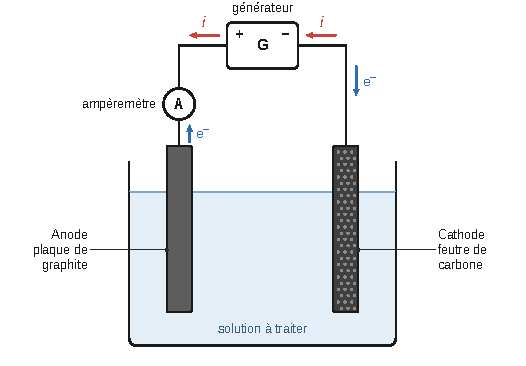
\includegraphics{figures/q3-montage-electro-fenton.pdf}
\caption*{Figure 1 --- dispositif électro-Fenton complété : générateur (borne +
vers l'anode), ampèremètre en série, sens des électrons et du courant i}
\end{figure}

Sens de déplacement des \textbf{électrons} : ils sont libérés à l'anode par l'oxydation et parcourent le fil de l'anode vers la borne + du générateur. Ils traversent le générateur, sortent par la borne − et rejoignent la cathode, où ils sont consommés.

Le courant \(i\) circule en sens inverse dans le circuit extérieur : il sort par la borne + vers l'anode. Dans la solution, le courant est assuré par la migration des ions (anions vers l'anode, cations vers la cathode), d'où le rôle d'électrolyte support de \(\mathrm{Na_2SO_4}\).

\hypertarget{q4}{%
\subsection{Q4}\label{q4}}

Montage à \textbf{trois électrodes} plongeant dans la solution étudiée, reliées à un potentiostat (ou à un générateur réglable, un voltmètre et un ampèremètre) :

\begin{itemize}
\tightlist
\item
  \textbf{électrode de travail} (carbone/graphite) : électrode étudiée, dont on impose le potentiel et dont on mesure le courant ;
\item
  \textbf{électrode de référence} (par exemple au calomel saturé) : potentiel fixe et connu ; le voltmètre (ou l'entrée haute impédance du potentiostat), branché entre elle et l'électrode de travail, mesure \(E\) ; elle n'est traversée par aucun courant ;
\item
  \textbf{contre-électrode} (électrode auxiliaire, par exemple en platine) : ferme le circuit ; l'ampèremètre, en série entre le générateur et la contre-électrode (ou l'électrode de travail), mesure \(i\).
\end{itemize}

\begin{figure}[H]
\centering
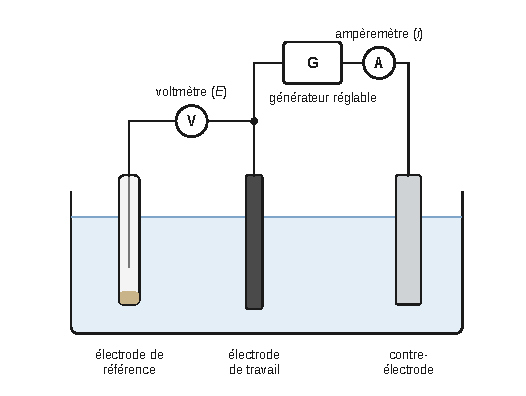
\includegraphics{figures/q4-montage-trois-electrodes.pdf}
\caption*{Figure 2 --- montage à trois électrodes : générateur réglable et
ampèremètre entre électrode de travail et contre-électrode, voltmètre
entre électrode de travail et électrode de référence}
\end{figure}

Le générateur réglable (ou le potentiostat) est la source qui permet de faire varier le potentiel de l'électrode de travail. On relève \(i\) point par point.

\hypertarget{q5}{%
\subsection{Q5}\label{q5}}

Espèces électroactives présentes : \(\mathrm{O_2}\) dissous, \(\mathrm{Fe^{2+}}\), le solvant (\(\mathrm{H_2O}\), \(\mathrm{H^+}\)). Pas de Fe³⁺ initialement, donc pas de vague de réduction du fer(III).

Les positions ci-dessous sont estimées à partir des potentiels standard (pH voisin de 0, le pH de la solution n'étant pas précisé). À pH 2, les vagues des couples faisant intervenir \(\mathrm{H^+}\) sont toutes décalées d'environ −0,12 V ; celle du fer ne bouge pas.

\begin{itemize}
\tightlist
\item
  Réduction \(\mathrm{O_2}\to\mathrm{H_2O_2}\) : système lent, vague décalée de −0,5 V par rapport à \(E^\circ=0{,}69\) V, vers \(0{,}2\) V. Palier de diffusion, car \(\mathrm{O_2}\) dissous est en faible concentration.
\item
  Oxydation \(\mathrm{Fe^{2+}}\to\mathrm{Fe^{3+}}\) : système rapide, vague centrée vers \(E^\circ\approx0{,}68\) V. Palier de diffusion (Fe²⁺ peu concentré).
\item
  Oxydation de l'eau : système lent, mur vers \(1{,}23+0{,}5\approx1{,}7\) V. Pas de palier : le solvant est en excès.
\item
  Réduction de \(\mathrm{H^+}\) : mur aux potentiels les plus bas (au voisinage de 0 V et en dessous).
\end{itemize}

\begin{figure}[H]
\centering
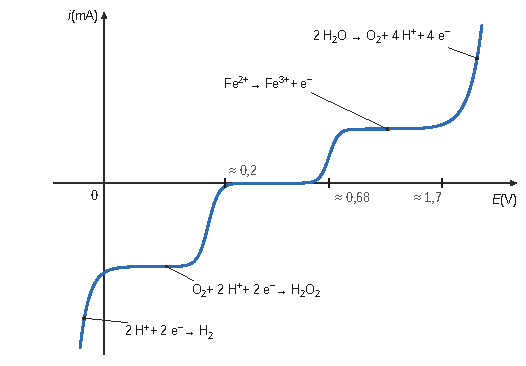
\includegraphics{figures/q5-courbe-intensite-potentiel.pdf}
\caption*{Figure 3 --- allure de la courbe intensité-potentiel annotée, axe des
potentiels non à l'échelle, i positif en oxydation}
\end{figure}

Courbe reproduite, de gauche à droite. Convention : \(i>0\) pour une oxydation (portions anodiques au-dessus de l'axe), \(i<0\) pour une réduction (portions cathodiques en dessous).

\begin{longtable}[]{@{}
  >{\raggedright\arraybackslash}p{(\columnwidth - 2\tabcolsep) * \real{0.4916}}
  >{\raggedright\arraybackslash}p{(\columnwidth - 2\tabcolsep) * \real{0.4784}}@{}}
\toprule\noalign{}
\begin{minipage}[b]{\linewidth}\raggedright
Portion de la courbe
\end{minipage} & \begin{minipage}[b]{\linewidth}\raggedright
Réaction électrochimique
\end{minipage} \\
\midrule\noalign{}
\endhead
\bottomrule\noalign{}
\endlastfoot
mur cathodique, \(i<0\) (\(E\) au voisinage de 0 V et en dessous) & \(2\,\mathrm{H^+}+2\,e^-\to\mathrm{H_2}\) \\
vague et palier cathodiques, \(i<0\) (vague vers 0,2 V) & \(\mathrm{O_2}+2\,\mathrm{H^+}+2\,e^-\to\mathrm{H_2O_2}\) \\
zone de courant nul (≈ 0,2 V à ≈ 0,6 V) & aucune réaction \\
vague et palier anodiques, \(i>0\) (vers 0,68 V) & \(\mathrm{Fe^{2+}}\to\mathrm{Fe^{3+}}+e^-\) \\
mur anodique, \(i>0\) (vers 1,7 V) & \(2\,\mathrm{H_2O}\to\mathrm{O_2}+4\,\mathrm{H^+}+4\,e^-\) \\
\end{longtable}

\hypertarget{q6}{%
\subsection{Q6}\label{q6}}

Il faut distinguer le potentiel de démarrage d'une réaction et le surpotentiel \(\eta\) : pour un système lent, la réaction démarre au potentiel \(E^\circ+\eta\), avec \(\eta<0\) à la cathode et \(\eta>0\) à l'anode.

À la cathode, la formation de \(\mathrm{H_2O_2}\) commence vers :

\equationajustee{E_c\approx E^\circ(\mathrm{O_2/H_2O_2})-0{,}5\approx0{,}2\ \mathrm{V}}

À l'anode, le dégagement de \(\mathrm{O_2}\) commence vers :

\equationajustee{E_a\approx E^\circ(\mathrm{O_2/H_2O})+0{,}5\approx1{,}7\ \mathrm{V}}

La tension minimale à appliquer est :

\equationajustee{\begin{aligned}
U_{\min}&=E_a-E_c\\
&\approx(1{,}23+0{,}5)-(0{,}69-0{,}5)\\
&\approx0{,}54+1{,}0
\end{aligned}}

\equationajustee{\boxed{U_{\min}\approx1{,}5\ \mathrm{V}}}

Elle ne dépend pas du pH : les deux couples échangent un \(\mathrm{H^+}\) par électron, et leurs potentiels varient tous deux de \(-0{,}06\) V par unité de pH. En pratique, il faut y ajouter la chute ohmique \(R\,i\) dans la solution.

\hypertarget{q7}{%
\subsection{Q7}\label{q7}}

Pour un élément des blocs s et p, le nombre d'électrons de valence se déduit de la colonne (colonne − 10 pour le bloc p) :

\begin{itemize}
\tightlist
\item
  N (2ᵉ ligne, 15ᵉ colonne : \(15-10\)) : \textbf{5 électrons de valence} ;
\item
  O (2ᵉ ligne, 16ᵉ colonne : \(16-10\)) : \textbf{6 électrons de valence} ;
\item
  S (3ᵉ ligne, même colonne que O, la 16ᵉ) : \textbf{6 électrons de valence}.
\end{itemize}

\hypertarget{q8}{%
\subsection{Q8}\label{q8}}

\textbf{Ion sulfate} \(\mathrm{SO_4^{2-}}\) : \(6+4\times6+2=32\) électrons, soit 16 doublets. Structure respectant l'octet : S central lié à quatre O par des liaisons simples, trois doublets non liants sur chaque O. Charges formelles : \(+2\) sur S et \(-1\) sur chaque O (total −2).

Écriture équivalente admise (S de la 3ᵉ période, hypervalence) : deux liaisons S=O et deux liaisons S--O⁻, charge formelle nulle sur S. Les quatre liaisons sont équivalentes par mésomérie (tétraèdre régulier).

\textbf{Ion ammonium} \(\mathrm{NH_4^+}\) : \(5+4-1=8\) électrons, 4 doublets. Quatre liaisons N--H, aucun doublet non liant, charge formelle \(+1\) sur N.

\textbf{Peroxyde d'hydrogène} \(\mathrm{H_2O_2}\) : \(2+12=14\) électrons, 7 doublets. Liaisons H--O, O--O, O--H et deux doublets non liants sur chaque O ; aucune charge formelle.

\begin{figure}[H]
\centering
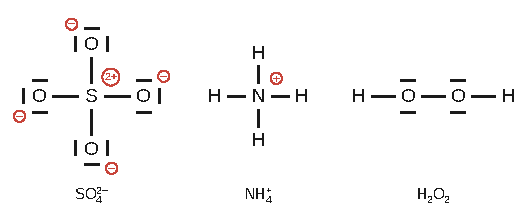
\includegraphics{figures/q8-lewis-sulfate-ammonium-peroxyde.pdf}
\caption*{Figure 4 --- schémas de Lewis de l'ion sulfate (octet, charges
formelles), de l'ion ammonium et du peroxyde d'hydrogène}
\end{figure}

\hypertarget{q9}{%
\subsection{Q9}\label{q9}}

Nombres d'oxydation du fer (O : −II, H : +I), notés \(x\) :

\begin{itemize}
\tightlist
\item
  \(\mathrm{Fe^{3+}}\) : +III ;
\item
  \(\mathrm{Fe(OH)_3}\) : \(x+3\times(-1)=0\), soit +III ;
\item
  \(\mathrm{Fe^{2+}}\) : +II ;
\item
  \(\mathrm{Fe(OH)_2}\) : \(x+2\times(-1)=0\), soit +II ;
\item
  \(\mathrm{Fe}\) : 0.
\end{itemize}

Verticalement, le nombre d'oxydation croît avec \(E\) : trois étages, +III en haut, +II au milieu, 0 en bas.

Horizontalement, à nombre d'oxydation donné, on classe les espèces par acidité. L'ion libre est la forme acide : \(\mathrm{Fe^{3+}}+3\,\mathrm{H_2O}=\mathrm{Fe(OH)_3}+3\,\mathrm{H^+}\) (de même pour Fe²⁺ et \(\mathrm{Fe(OH)_2}\)). L'hydroxyde, forme basique, occupe donc les pH élevés, et l'ion libre les pH faibles.

\begin{longtable}[]{@{}lll@{}}
\toprule\noalign{}
Domaine & Espèce & n.o. du fer \\
\midrule\noalign{}
\endhead
\bottomrule\noalign{}
\endlastfoot
\textbf{A} & \(\mathrm{Fe^{3+}_{(aq)}}\) & +III \\
\textbf{B} & \(\mathrm{Fe(OH)_{3(s)}}\) & +III \\
\textbf{C} & \(\mathrm{Fe^{2+}_{(aq)}}\) & +II \\
\textbf{D} & \(\mathrm{Fe(OH)_{2(s)}}\) & +II \\
\textbf{E} & \(\mathrm{Fe_{(s)}}\) & 0 \\
\end{longtable}

Contrôles sur les frontières :

\begin{itemize}
\tightlist
\item
  A/C est horizontale (Fe³⁺ + e⁻ = Fe²⁺, sans H⁺) ;
\item
  A/B et C/D sont verticales (précipitations, pH ≈ 1,7 et ≈ 7) ;
\item
  B/C a une pente de \(-0{,}18\) V/pH (\(\mathrm{Fe(OH)_3}+3\,\mathrm{H^+}+e^-=\mathrm{Fe^{2+}}+3\,\mathrm{H_2O}\)) ;
\item
  B/D et D/E ont une pente de \(-0{,}06\) V/pH.
\end{itemize}

Les frontières verticales correspondent à une concentration de tracé de \(10^{-1}\) mol·L⁻¹ : \(14-(38-1)/3\approx1{,}7\) et \(14-(15-1)/2=7\).

\hypertarget{q10}{%
\subsection{Q10}\label{q10}}

Seul le sel de Mohr apporte Fe²⁺ :

\equationajustee{n=4{,}5\cdot10^{-3}\times10\cdot10^{-3}=4{,}5\cdot10^{-5}\ \mathrm{mol}}

Volume total (gouttes d'acide et volume du solide négligés) : \(V=170+10=180\) mL. Par conservation de la quantité de fer(II) lors de la dilution :

\equationajustee{C_0=\frac{n}{V}=\frac{4{,}5\cdot10^{-5}}{0{,}180}}

\equationajustee{\boxed{C_0=2{,}5\cdot10^{-4}\ \mathrm{mol\cdot L^{-1}}}}

\hypertarget{q11}{%
\subsection{Q11}\label{q11}}

Équilibre de dissolution : \(\mathrm{Fe(OH)_{3(s)}}=\mathrm{Fe^{3+}_{(aq)}}+3\,\mathrm{HO^-_{(aq)}}\). Le précipité apparaît quand le quotient de réaction atteint \(K_s\), tout le fer(III) étant encore dissous :

\equationajustee{Q^{eq}=\frac{[\mathrm{Fe^{3+}}]\,[\mathrm{HO^-}]^3}{(c^\circ)^4}=K_s}

\equationajustee{K_s=10^{-\mathrm{p}K_s}=10^{-38}}

avec \([\mathrm{Fe^{3+}}]=C_0'=1{,}0\cdot10^{-4}\) mol·L⁻¹. D'où :

\equationajustee{\begin{aligned}
\log\frac{[\mathrm{HO^-}]}{c^\circ}&=\frac{1}{3}\left(-\mathrm{p}K_s-\log\frac{C_0'}{c^\circ}\right)=\frac{-38+4}{3}\\
\mathrm{pOH}&=\frac{34}{3}\approx11{,}3\\
\mathrm{pH}&=\mathrm{p}K_e-\mathrm{pOH}\approx14-11{,}3
\end{aligned}}

\equationajustee{\boxed{\mathrm{pH}\approx2{,}7}}

Au-dessus de pH 2,7, \(\mathrm{Fe(OH)_3}\) précipite ; en dessous, le fer(III) reste dissous. L'expérience est menée à pH = 2 \textless{} 2,7 : le fer(III) ne précipite pas. Il reste en solution, peut être réduit en Fe²⁺ à la cathode et entretenir le cycle de Fenton. \textbf{Les conditions de pH sont donc cohérentes avec le procédé.}

Même si tout le fer du bécher était à l'état +III, \([\mathrm{Fe^{3+}}]=2{,}5\cdot10^{-4}\) mol·L⁻¹ donnerait un pH de début de précipitation ≈ 2,5, encore supérieur à 2.

\hypertarget{q12}{%
\subsection{Q12}\label{q12}}

On règle le spectrophotomètre au \textbf{maximum d'absorption} du bleu de méthylène, lu sur l'annexe 6 :

\equationajustee{\boxed{\lambda\approx665\ \mathrm{nm}}}

(un maximum secondaire, plus bas, apparaît vers 620 nm). Justification :

\begin{itemize}
\tightlist
\item
  \(\varepsilon\) y est maximal, donc la sensibilité est maximale ;
\item
  au voisinage d'un maximum, \(A\) varie peu avec \(\lambda\), d'où une mesure peu sensible à un léger défaut de réglage ;
\item
  le BM étant la seule espèce colorée, l'absorbance ne mesure que lui.
\end{itemize}

\hypertarget{q13}{%
\subsection{Q13}\label{q13}}

L'absorbance est proportionnelle à \([\mathrm{BM}]\) (seule espèce colorée) : \(t_{1/2}\) est l'instant où \(A=A_0/2=0{,}937\).

D'après le tableau, \(A(240)=0{,}993\) et \(A(300)=0{,}863\) encadrent 0,937. Par interpolation linéaire :

\equationajustee{\begin{aligned}
t_{1/2}&\approx240+60\times\frac{0{,}993-0{,}937}{0{,}993-0{,}863}\\
&\approx240+26
\end{aligned}}

\equationajustee{\boxed{t_{1/2}\approx2{,}7\cdot10^{2}\ \mathrm{s}}}

(soit environ 4,5 min ; encadrement sûr : 240 s \textless{} \(t_{1/2}\) \textless{} 300 s).

\hypertarget{q14}{%
\subsection{Q14}\label{q14}}

Pour une solution d'une espèce absorbante traversée par une lumière monochromatique de longueur d'onde \(\lambda\) :

\equationajustee{\boxed{A=\log\frac{I_0}{I}=\varepsilon_\lambda\,\ell\,c}}

\begin{itemize}
\tightlist
\item
  \(A\) : absorbance, sans dimension (\(I_0\) intensité incidente, \(I\) intensité transmise) ;
\item
  \(\varepsilon_\lambda\) : coefficient d'absorption molaire, en L·mol⁻¹·cm⁻¹ ;
\item
  \(\ell\) : longueur de solution traversée (épaisseur de la cuve), en cm ;
\item
  \(c\) : concentration de l'espèce absorbante, en mol·L⁻¹.
\end{itemize}

Valable pour des solutions diluées ; les absorbances de plusieurs espèces s'ajoutent.

\hypertarget{q15}{%
\subsection{Q15}\label{q15}}

Loi de vitesse d'ordre 1, puis séparation des variables et intégration entre 0 et \(t\) :

\equationajustee{\begin{aligned}
v=-\frac{\mathrm{d}[\mathrm{BM}]}{\mathrm{d}t}&=k[\mathrm{BM}]\\
\frac{\mathrm{d}[\mathrm{BM}]}{[\mathrm{BM}]}&=-k\,\mathrm{d}t\\
\ln\frac{[\mathrm{BM}](t)}{[\mathrm{BM}]_0}&=-k\,t
\end{aligned}}

Par Beer-Lambert (BM seule espèce colorée, \(\lambda\) et cuve fixées), \(A=\varepsilon\ell[\mathrm{BM}]\) et \(A_0=\varepsilon\ell[\mathrm{BM}]_0\). Le rapport des concentrations est donc celui des absorbances :

\equationajustee{\boxed{\ln A=\ln A_0-k\,t}}

soit, de façon équivalente :

\equationajustee{A(t)=A_0\,{\mathrm{e}}^{-kt}}

\hypertarget{q16}{%
\subsection{Q16}\label{q16}}

Si la réaction est d'ordre 1, la question 15 prévoit que \(\ln A\) est une fonction affine décroissante de \(t\), de pente \(-k\).

Sur la figure 5, les points \(\ln A\) en fonction de \(t\) (en s) sont bien alignés sur la droite de régression \(y=-2{,}23\cdot10^{-3}x+0{,}563\), sur tout le domaine étudié (0 à 600 s) : \textbf{l'allure justifie l'ordre 1} (elle est compatible avec lui).

Par identification de la pente \(-k\) :

\equationajustee{\boxed{k=2{,}23\cdot10^{-3}\ \mathrm{s^{-1}}}}

Nuance : les \(\ln A\) calculés à partir du tableau 1 s'écartent un peu de la droite aux extrémités (0,63 à \(t=0\) contre 0,563 ; −0,70 à \(t=600\) s contre −0,78). L'ordonnée à l'origine donne ainsi \({\mathrm{e}}^{0{,}563}\approx1{,}76\) au lieu de \(A_0=1{,}873\). L'accord reste satisfaisant.

\hypertarget{q17}{%
\subsection{Q17}\label{q17}}

Éliminer 99 \% du BM, c'est atteindre \(A/A_0=10^{-2}\). D'après la question 15 :

\equationajustee{\begin{aligned}
t_{99}&=\frac{1}{k}\ln\frac{A_0}{A}=\frac{2\ln10}{k}\\
&\approx\frac{4{,}6}{2{,}23\cdot10^{-3}}
\end{aligned}}

\equationajustee{\boxed{t_{99}\approx2{,}1\cdot10^{3}\ \mathrm{s}\approx34\ \mathrm{min}}}

Durée positive, comme il se doit : \(\ln(A_0/A)=\ln100>0\). L'expérience de 10 min ne dégrade donc qu'environ 74 \% du colorant (\(0{,}495/1{,}873\approx0{,}26\) restant).

\hypertarget{q18}{%
\subsection{Q18}\label{q18}}

Maille conventionnelle CFC : cube d'arête \(a\), atomes aux 8 sommets et aux centres des 6 faces.

\begin{figure}[H]
\centering
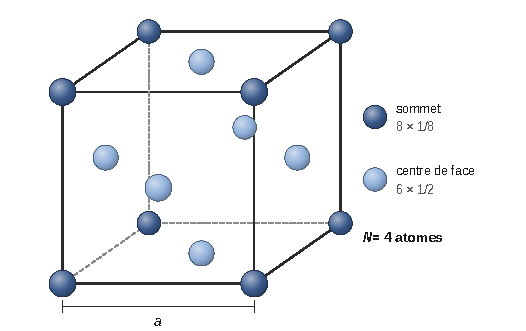
\includegraphics{figures/q18-maille-cfc.pdf}
\caption*{Figure 5 --- maille conventionnelle CFC du platine : 8 atomes aux
sommets comptés 1/8, 6 aux centres des faces comptés 1/2}
\end{figure}

\begin{itemize}
\tightlist
\item
  Population : \(N=8\times\frac18+6\times\frac12=\boxed{4\ \text{atomes par maille}}\).
\item
  Coordinence (nombre de plus proches voisins d'un atome, à ne pas confondre avec la compacité) : un atome au centre d'une face a pour plus proches voisins, à la distance \(a/\sqrt2\), les 4 sommets de cette face et 4 centres de faces dans chacune des deux mailles qui partagent cette face : \(\boxed{12}\).
\end{itemize}

\hypertarget{q19}{%
\subsection{Q19}\label{q19}}

Les atomes sont tangents le long de la diagonale d'une face (sommet, centre de face, sommet) : \(a\sqrt2=4R\), donc \(a=2\sqrt2\,R\).

\begin{figure}[H]
\centering
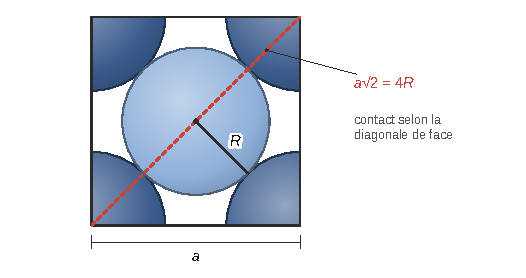
\includegraphics{figures/q19-contact-diagonale-face.pdf}
\caption*{Figure 6 --- face de la maille CFC : contact des atomes le long de la
diagonale, a√2 = 4R}
\end{figure}

Avec \(\sqrt2\approx10/7\) :

\equationajustee{a\approx2\times\frac{10}{7}\times140\ \mathrm{pm}}

\equationajustee{\boxed{a\approx4{,}0\cdot10^{2}\ \mathrm{pm}=4{,}0\cdot10^{-10}\ \mathrm{m}}}

(La valeur sans approximation est 396 pm.)

\hypertarget{q20}{%
\subsection{Q20}\label{q20}}

Masse des \(N\) atomes d'une maille divisée par le volume \(a^3\) de la maille, en unités SI :

\equationajustee{\begin{aligned}
\rho&=\frac{N\,M(\mathrm{Pt})}{{\mathcal{N}}_A\,a^3}\\
&=\frac{4\times200\cdot10^{-3}}{6\cdot10^{23}\times(4{,}0\cdot10^{-10})^3}\\
&=\frac{0{,}8}{6\times64\cdot10^{-7}}\\
&=\frac{0{,}8}{3{,}84\cdot10^{-5}}\ \mathrm{kg\cdot m^{-3}}
\end{aligned}}

\equationajustee{\boxed{\rho\approx2{,}1\cdot10^{4}\ \mathrm{kg\cdot m^{-3}}=21\ \mathrm{g\cdot cm^{-3}}}}

Valeur conforme à la masse volumique tabulée du platine (21,4 g·cm⁻³).

\hypertarget{traitement-des-eaux-par-des-procuxe9duxe9s-biologiques}{%
\section{Traitement des eaux par des procédés biologiques}\label{traitement-des-eaux-par-des-procuxe9duxe9s-biologiques}}

\hypertarget{traitement-des-eaux-en-milieu-auxe9robie}{%
\subsection{Traitement des eaux en milieu aérobie}\label{traitement-des-eaux-en-milieu-auxe9robie}}

\hypertarget{q21}{%
\subsection{Q21}\label{q21}}

Bilan C, puis H, puis O :

\equationajustee{\boxed{\mathrm{C_2H_6O_{(aq)}}+3\,\mathrm{O_{2(aq)}}\longrightarrow2\,\mathrm{CO_{2(g)}}+3\,\mathrm{H_2O_{(\ell)}}}}

(C : 2 = 2 ; H : 6 = 6 ; O : 1 + 6 = 4 + 3.)

\hypertarget{q22}{%
\subsection{Q22}\label{q22}}

Loi de Hess avec les données de l'annexe 5 (O₂ dissous : \(\Delta_fH^\circ\) et \(S_m^\circ\) non nuls) :

\equationajustee{\Delta_rH^\circ=2(-400)+3(-300)-(-300)-3(-10)=-1370\ \mathrm{kJ\cdot mol^{-1}}}

\equationajustee{\Delta_rS^\circ=2(200)+3(50)-150-3(100)=+100\ \mathrm{J\cdot K^{-1}\cdot mol^{-1}}}

\equationajustee{\begin{aligned}
\Delta_rG^\circ&=\Delta_rH^\circ-T\Delta_rS^\circ\\
&=-1370-298\times0{,}100\\
&\approx-1370-30\ \mathrm{kJ\cdot mol^{-1}}
\end{aligned}}

\equationajustee{\boxed{\Delta_rG^\circ\approx-1{,}40\cdot10^{3}\ \mathrm{kJ\cdot mol^{-1}}}}

De \(\Delta_rG^\circ=-RT\ln K_1^\circ\) :

\equationajustee{\begin{aligned}
\ln K_1^\circ&=-\frac{\Delta_rG^\circ}{RT}=\frac{1{,}40\cdot10^{6}}{8\times298}\approx5{,}9\cdot10^{2}\\
\log K_1^\circ&=\frac{\ln K_1^\circ}{\ln10}\approx\frac{587}{2{,}3}\approx255
\end{aligned}}

\equationajustee{\boxed{K_1^\circ\approx10^{255}}}

Conclusion : \(K_1^\circ\gg10^4\), la réaction est \textbf{thermodynamiquement totale} ; l'éthanol peut être entièrement minéralisé par le dioxygène dissous. Elle est en revanche lente sans catalyseur : ce sont les bactéries (leurs enzymes) qui la rendent effective.

\hypertarget{traitement-des-eaux-en-milieu-anauxe9robie-duxe9pourvu-doxyguxe8ne}{%
\subsection{Traitement des eaux en milieu anaérobie (dépourvu d'oxygène)}\label{traitement-des-eaux-en-milieu-anauxe9robie-duxe9pourvu-doxyguxe8ne}}

\hypertarget{q23}{%
\subsection{Q23}\label{q23}}

La somme des nombres d'oxydation vaut la charge de l'ion, avec O à −II :

\equationajustee{x+3\times(-2)=-1}

donc \(\boxed{\mathrm{n.o.(N)}=+\mathrm{V}}\) dans \(\mathrm{NO_3^-}\).

\hypertarget{q24}{%
\subsection{Q24}\label{q24}}

\equationajustee{\boxed{2\,\mathrm{NO^-_{3(aq)}}+12\,\mathrm{H^+_{(aq)}}+10\,e^-=\mathrm{N_{2(g)}}+6\,\mathrm{H_2O_{(\ell)}}}}

(N : +V → 0, \(2\times5=10\) électrons ; charges : \(-2+12-10=0\).)

Relation de Nernst : l'oxydant \(\mathrm{NO_3^-}\) et les \(\mathrm{H^+}\) (côté oxydant) au numérateur, le réducteur \(\mathrm{N_2}\) au dénominateur, l'eau (solvant) n'apparaît pas :

\equationajustee{\boxed{E_1=E^\circ(\mathrm{NO_3^-/N_2})+\frac{0{,}06}{10}\log\frac{[\mathrm{NO_3^-}]^2\,[\mathrm{H^+}]^{12}}{(c^\circ)^{14}\,\dfrac{p_{\mathrm{N_2}}}{p^\circ}}}}

avec \(E^\circ=1{,}25\) V. Sous forme développée (en V) :

\equationajustee{E_1=1{,}25+0{,}012\log\frac{[\mathrm{NO_3^-}]}{c^\circ}-0{,}072\,\mathrm{pH}-0{,}006\log\frac{p_{\mathrm{N_2}}}{p^\circ}}

\hypertarget{q25}{%
\subsection{Q25}\label{q25}}

\equationajustee{\boxed{2\,\mathrm{CO_{2(g)}}+12\,\mathrm{H^+_{(aq)}}+12\,e^-=\mathrm{C_2H_6O_{(aq)}}+3\,\mathrm{H_2O_{(\ell)}}}}

(C : +IV → −II en moyenne, \(2\times6=12\) électrons.)

L'oxydant est \(\mathrm{CO_2}\) (numérateur, avec les \(\mathrm{H^+}\)), le réducteur l'éthanol (dénominateur) :

\equationajustee{\boxed{E_2=E^\circ(\mathrm{CO_2/C_2H_6O})+\frac{0{,}06}{12}\log\frac{\left(\dfrac{p_{\mathrm{CO_2}}}{p^\circ}\right)^2[\mathrm{H^+}]^{12}}{[\mathrm{C_2H_6O}]\,(c^\circ)^{11}}}}

avec \(E^\circ=-0{,}33\) V. Sous forme développée (en V) :

\equationajustee{E_2=-0{,}33+0{,}01\log\frac{p_{\mathrm{CO_2}}}{p^\circ}-0{,}06\,\mathrm{pH}-0{,}005\log\frac{[\mathrm{C_2H_6O}]}{c^\circ}}

\hypertarget{q26}{%
\subsection{Q26}\label{q26}}

\(E^\circ(\mathrm{NO_3^-/N_2})=1{,}25\) V est supérieur à \(E^\circ(\mathrm{CO_2/C_2H_6O})=-0{,}33\) V : le nitrate oxyde l'éthanol. On combine \(6\times\)(Q24) et \(5\times\)(Q25 dans le sens de l'oxydation), soit 60 électrons échangés :

\equationajustee{\boxed{5\,\mathrm{C_2H_6O_{(aq)}}+12\,\mathrm{NO^-_{3(aq)}}+12\,\mathrm{H^+_{(aq)}}=10\,\mathrm{CO_{2(g)}}+6\,\mathrm{N_{2(g)}}+21\,\mathrm{H_2O_{(\ell)}}}}

(C 10 = 10 ; N 12 = 12 ; H 42 = 42 ; O 41 = 41 ; charges 0 = 0.)

À l'équilibre \(E_1=E_2\), d'où, avec \(n=60\) :

\equationajustee{\begin{aligned}
\log K_2^\circ&=\frac{n\,(E_1^\circ-E_2^\circ)}{0{,}06}\\
&=\frac{60\times1{,}58}{0{,}06}=1580
\end{aligned}}

\equationajustee{\boxed{K_2^\circ\approx10^{1580}}}

(Pour l'équation rapportée à une mole d'éthanol, \(n=12\) et \(K^\circ=10^{316}\).)

Conclusion : la réaction est \textbf{totale} ; en l'absence de dioxygène, les ions nitrate oxydent quantitativement l'éthanol en \(\mathrm{CO_2}\) et sont éliminés sous forme de diazote gazeux (dénitrification). Comme en milieu aérobie, la réaction est lente sans catalyse bactérienne.

\end{document}
